\section{Data and exploratory analysis}
\label{sec:data-eda}

Before fitting return models, we build a clean ten-year panel of Oslo Stock
Exchange equities and examine the main patterns in their daily returns. These
empirical features define what our risk models need to reproduce.

\subsection{Data source}
\label{sec:data-source}

The stock data come from TITLON, a financial database for Norwegian academic
institutions \parencite{TITLON}. The raw export contains 1,876,617 daily
records for 1,133 ISINs\footnote{An International Securities Identification
Number (ISIN) identifies a security, such as a share class.}, spanning
2 January 1980 to 8 September 2026. From this export, we focus on a ten-year
sample of 2,510 trading days on the Oslo Stock Exchange (XOSL), from
8 September 2016 to 8 September 2026. All prices and turnover are recorded in
Norwegian kroner (NOK).

\subsection{Data preparation}
\label{sec:data-preparation}

Turning the raw export into a consistent return panel requires cleaning split
histories, adjusting for corporate actions, filtering for data coverage, and
handling short missing-price gaps.

Some share classes appear under different ISINs over time, splitting their
price histories, while a company can also have multiple share classes trading
under different ISINs at the same time. We reconstruct one price series per
share class by joining nonoverlapping histories when known ISIN links or
identifiers in the data indicate continuity, while keeping concurrently traded
classes separate. Duplicate prices for the same stock and day are counted once;
if duplicates disagree, or if a price is zero, negative, or nonfinite, the
price is treated as missing.

Stock splits and dividends can lower the share price while leaving the
shareholder's total value unchanged. We therefore work with TITLON's
\texttt{AdjustedPrice} column, given by
\mbox{\(P^{*}=\texttt{Price}\times\texttt{CorpAdj}\times\texttt{DividendAdj}\)}.
Here, \texttt{Price} is the recorded share price, \texttt{CorpAdj} adjusts for
corporate actions such as splits, and \texttt{DividendAdj} adjusts for dividends
\parencite{TITLONFields}. Figure~\ref{fig:kongsberg-adjusted-price} illustrates
this for Kongsberg Gruppen around its five-for-one split on 3 June 2025
\parencite[154]{KongsbergAnnualReport2025}: from 2 to 3 June, the recorded
price fell by 79.5\%, whereas the adjusted price rose by 2.7\%.

\begin{figure}[H]
    \centering
    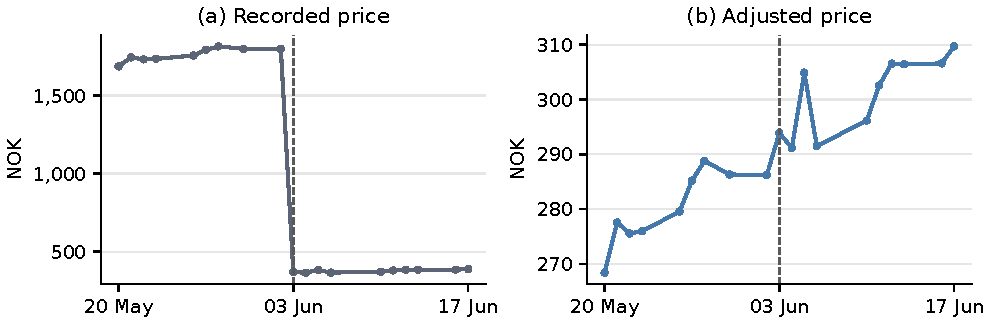
\includegraphics[width=\linewidth]{figures/data/kongsberg-adjusted-price.pdf}
    \caption{Kongsberg Gruppen's recorded and adjusted share prices from
    20 May to 17 June 2025, using TITLON data. The dashed line marks the
    split. The panels use different vertical scales.}
    \label{fig:kongsberg-adjusted-price}
\end{figure}

To avoid counting the same company twice, we select one share class per
company, choosing the class with the most valid adjusted prices. Ties are
broken by higher total turnover in NOK over the sample period, then by the
lowest final ISIN. From the resulting 115 candidate histories, we keep only
stocks with a valid adjusted price on 8 September 2026 (the final trading day),
valid prices on more than 95\% of trading days, and gaps of at most five
consecutive trading days. This leaves a final sample of 111 stocks.

Before calculating returns, we fill internal gaps of up to five trading days
in each stock's adjusted prices. We fit a natural cubic spline to the
observed prices using trading-day positions and fill a gap only when all
estimated prices are finite and positive. Because the spline uses prices on
both sides of the gap, these estimates are retrospective.

Daily log returns are then calculated as
\begin{equation}
    r_{i,t}=\log P^{*}_{i,t}-\log P^{*}_{i,t-1},
    \label{eq:eda-log-return}
\end{equation}
where \(t-1\) is the previous trading day. The first possible return falls on
the second trading day of the sample, and a return remains missing if either
price is still missing. We use log returns for modelling because they are
unbounded on \((-\infty,\infty)\) and additive over time, which matches the
additive structure of stochastic differential equations and guarantees positive
prices. Because portfolio returns combine linearly in simple returns rather
than log returns, we convert daily log returns back to simple returns via
\(R_{i,t}=e^{r_{i,t}}-1\) before applying portfolio weights and compounding
over multi-day horizons in portfolio risk calculations.

Interpolation fills all 1,222 missing prices between observed prices, leaving
only three prices missing on 8 September 2016 where no earlier observations
exist in the sample. The interpolated prices provide estimates for 2,259 of the
2,262 missing returns after the first trading day and increase the number of
days with returns for all 111 stocks from 1,688 to 2,507. Using all available
returns for each stock and weighting stocks equally, the average daily return
variance decreases by 0.49\%.

Finally, to compare stocks within and across industries, we match each of the
111 retained stocks by its final ISIN to Euronext's 17 November 2026 Industry
Classification Benchmark (ICB) snapshot and keep that Industry label throughout
the sample \parencite{EuronextOsloEquities}. Table~\ref{tab:eda-sectors} shows
the resulting sample composition by ICB Industry. ICB also classifies stocks at
the more detailed Supersector and Sector levels;
Tables~\ref{tab:icb-supersector-counts} and~\ref{tab:icb-sector-counts} in
Appendix~\ref{app:icb-sample-composition} give the counts at those levels.

\begin{table}[htbp]
    \centering
    \caption{Sample composition by ICB Industry.}
    \label{tab:eda-sectors}
    \small
    \begin{tabular}{lr@{\hspace{1cm}}lr}
        \hline
        Industry & Stocks & Industry & Stocks \\
        \hline
        Basic Materials & 4 & Industrials & 22 \\
        Consumer Discretionary & 6 & Real Estate & 2 \\
        Consumer Staples & 9 & Technology & 11 \\
        Energy & 28 & Telecommunications & 2 \\
        Financials & 19 & Utilities & 1 \\
        Health Care & 7 & & \\
        \hline
        \multicolumn{3}{r}{Total} & 111 \\
        \hline
    \end{tabular}
\end{table}

\subsection{Exploratory analysis}
\label{sec:exploratory-analysis}

With the ten-year return panel in place, we examine three empirical patterns
that matter for portfolio risk modelling: heavy tails, changing volatility, and
stronger dependence within industries.

First, daily returns have heavier tails than a normal distribution.
Figure~\ref{fig:eda-return-behaviour}a compares standardized returns with a
normal reference after scaling each stock separately to remove differences in
overall volatility. Both large losses and large gains occur more often than a
normal distribution predicts, showing that simple normal assumptions
underestimate extreme moves.

\begin{figure}[htbp]
    \centering
    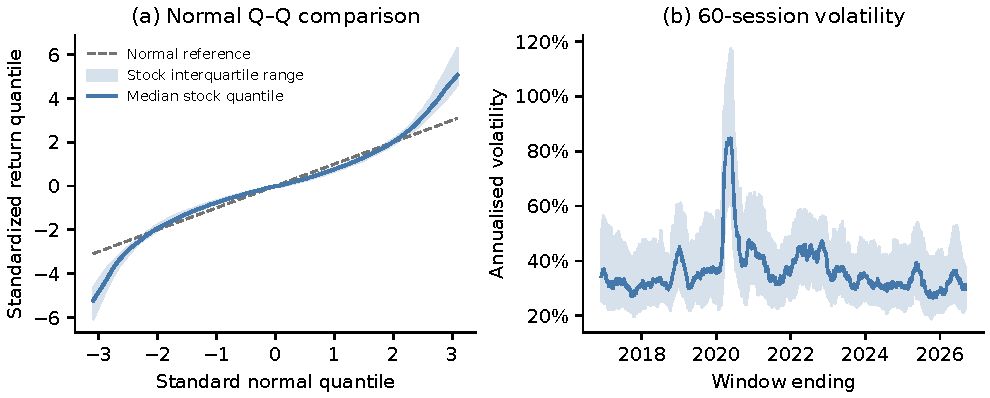
\includegraphics[width=\linewidth]{figures/data/return-behaviour.pdf}
    \caption{Returns and volatility over the ten-year sample after short-gap
    interpolation. (a) Comparison with a normal distribution after subtracting
    each stock's mean return and dividing by its standard deviation. The curve
    shows the median across stocks; the band covers the middle 50\%.
    (b) Volatility measured over 60 trading days and converted to an annual
    scale using \(\sqrt{252}\). Each estimate requires 60 consecutive daily returns.
    The line shows the median across stocks; the band covers the middle 50\%.
    These bands show differences between stocks, not uncertainty intervals.}
    \label{fig:eda-return-behaviour}
\end{figure}

Second, volatility changes strongly over time rather than staying constant.
Figure~\ref{fig:eda-return-behaviour}b shows that the market shifts between
calmer and much more turbulent periods, while volatility levels also vary
widely across stocks. Models that assume constant volatility therefore miss
how risk builds up during stressed periods.

Third, stocks in the same ICB Industry tend to move together more closely than
stocks in different industries. Using shared dates for each stock pair, average
Pearson correlation is 0.169 within industries and 0.109 across industries. The
within-group average rises to 0.170 at the Supersector level and to 0.193 at
the Sector level. As Figure~\ref{fig:eda-dependence}a shows, within-industry
correlation remains higher than across-industry correlation throughout the
sample, while both fluctuate noticeably over time.

\begin{figure}[htbp]
    \centering
    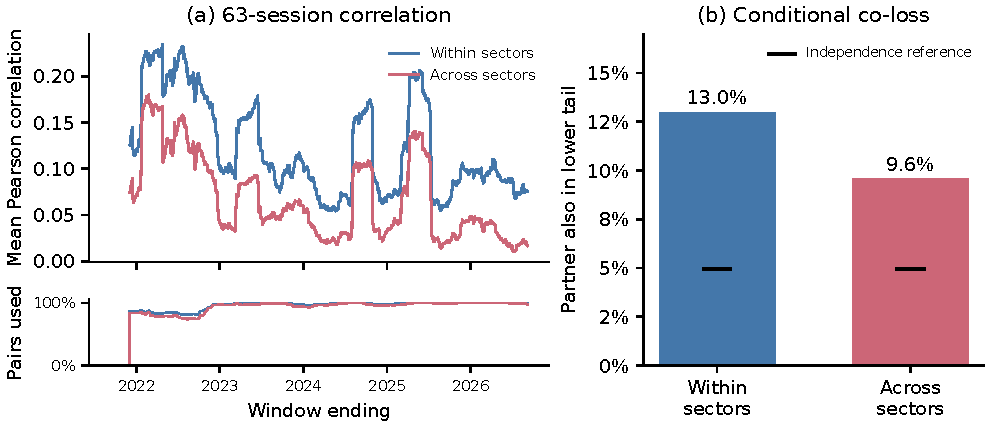
\includegraphics[width=\linewidth]{figures/data/dependence-and-losses.pdf}
    \caption{Links between stock returns in the selected sample.
    (a) Average Pearson correlations within and across industries, measured over
    63 trading days. Each stock pair needs returns for all 63 days. The lower
    strip shows the share of eligible pairs included.
    (b) Average chance that a stock has one of its worst 5\% of returns when
    another stock does, using their shared dates and averaging both directions.
    Black markers show the reference values for independent returns, allowing
    for tied values. The bars show averages, without uncertainty intervals.}
    \label{fig:eda-dependence}
\end{figure}

Large losses also occur together much more often than under independence,
especially within the same industry. When one stock has one of its worst 5\% of
returns, another stock does too on average 17.6\% of the time within
industries, compared with 13.8\% across industries
(Figure~\ref{fig:eda-dependence}b).

\subsection{Correlation spikes during market shocks}
\label{sec:eda-implications}

While full-sample averages show stronger links within industries, they still
hide sharp short-term jumps during large market moves. When a broad market
shock hits, whether a sharp sell-off or a strong rebound, correlations can
spike both within and across industries as stocks that usually move fairly
independently begin moving together. Figure~\ref{fig:eda-correlation-shocks}
illustrates this in two episodes, plotting rolling 20-day average correlations
alongside the median daily stock return.

The first episode is January 2022, when concerns about higher interest rates and
tensions between Russia and Ukraine weighed on equity markets
\parencite{FOMCJanuary2022}. From 21 to 24 January, average correlation jumped
from 0.23 to 0.35 within industries and from 0.15 to 0.30 across industries,
and rose further during the sharp rebound two days later. The second episode is
the global sell-off in early August 2024 \parencite{AquilinaEtAl2024}. From 1 to
5 August, average correlation rose from 0.07 to 0.34 within industries and from
0.03 to 0.27 across industries.

\begin{figure}[htbp]
    \centering
    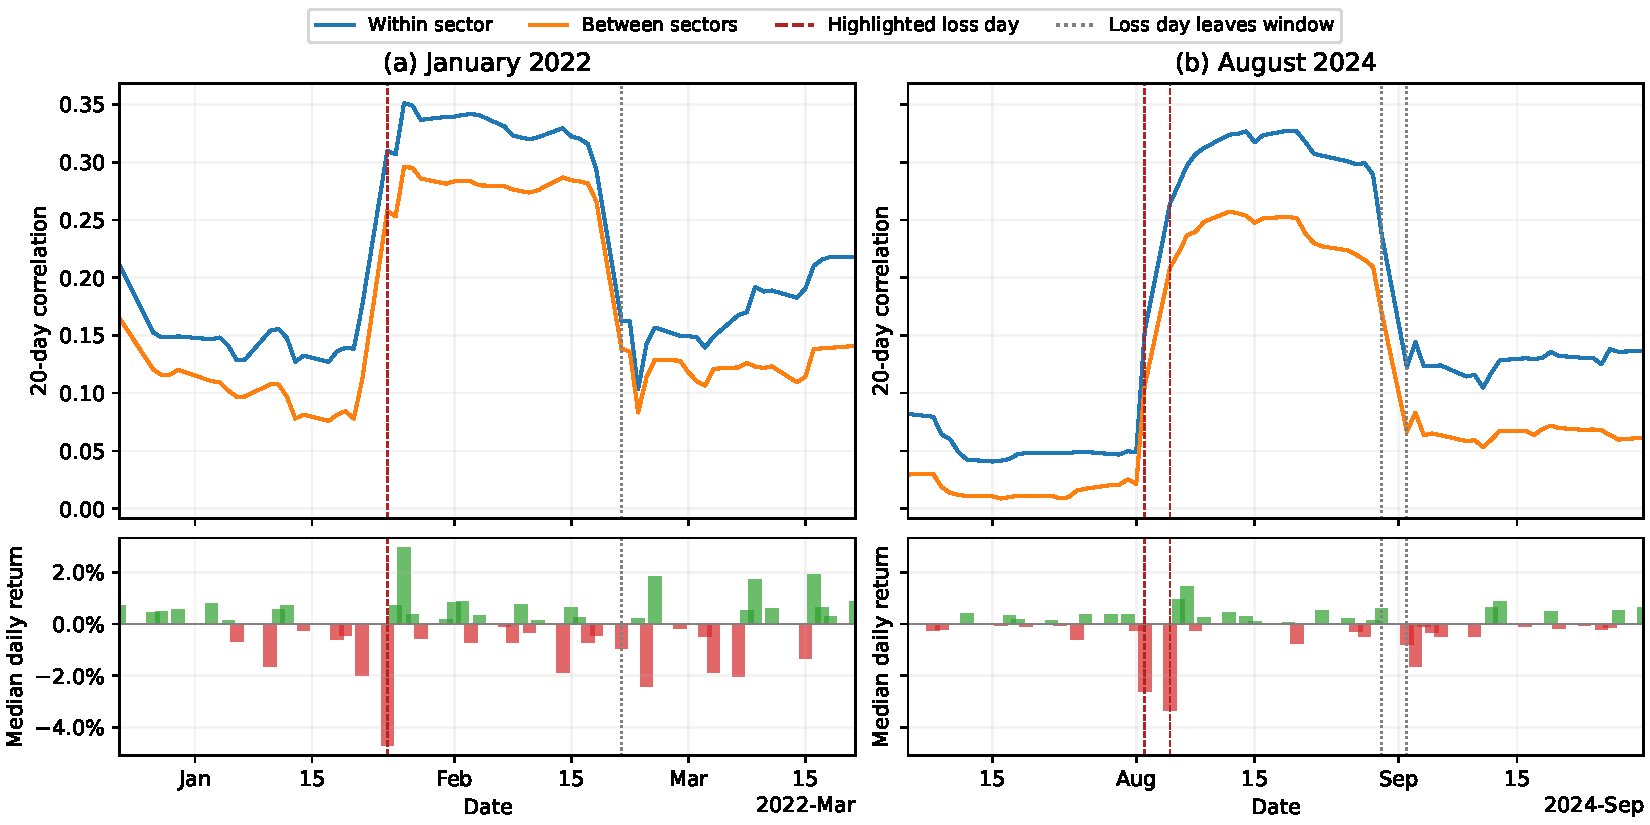
\includegraphics[width=\linewidth]{figures/data/correlation-shocks.pdf}
    \caption{Correlation jumps in January 2022 and August 2024. The upper panels
    show average Pearson correlations over the previous 20 trading days, using
    stocks with returns on every day in the window. The lower panels show the
    median daily stock return. Red dashed lines mark the highlighted shock days;
    grey dotted lines mark when those days leave the 20-day window.}
    \label{fig:eda-correlation-shocks}
\end{figure}

Rolling 20-day correlations should be read with care. A single large market-wide
move lifts the estimate for as long as it stays in the 20-day window, and
correlations fall back once that day leaves the window (grey dotted lines).
These examples therefore show how strongly short-term correlations react to a
few large shared moves, rather than proving that every market shock behaves the
same way.

Taken together, the exploratory analysis highlights four features that a
realistic risk model needs to handle: heavy tails, changing volatility,
cross-stock dependence with joint losses, and sharp correlation spikes during
large market moves. Matching only long-run averages misses how co-movement
shifts during turbulent periods. This motivates copula models, which separate
how stocks move together from each stock's own return distribution. It also
raises a key question for this thesis: is a fixed copula enough, or do we need
a dynamic or conditional neural SDE that lets both volatility and dependence
change with market conditions?
